%\chapterauthor{Author Name}{Author Affiliation}
%\chapterauthor{Second Author}{Second Author Affiliation}
\chapter{Storage Management}

Upon installation of the system, the OS shall scan the machine, look for hard drives, and either automatically or manually partition it into partitions and mount the partitions to different locations in the OS such as \verb|/| (root directory), \verb|/home/|, swap space, etc.

It is often not necessary for a casual user to manage the partitions and mountings by himself as there is the option to let Linux installation handle them automatically. However, when comes to Linux servers where hardware and storage is scaled up and down frequently, it is recommended that the administrator shall understand how hard drive can be managed. Linux provides flexible tools to monitor and manage the storage of the machine, including manipulating partition table, format partition, and managing its mounting point.

\section{Partitions and Filesystems}

A partition is a logical slice of the hard drive managed by the OS via partition table which is introduced in more details in a later stage. A filesystem, on the other hand, reflects how OS formats data in the partition and where it is mounted in the OS filesystem hierarchy. This is demonstrated by Fig. \ref{ch:dm:fig:partition}.

\begin{figure}[htbp]
	\centering
	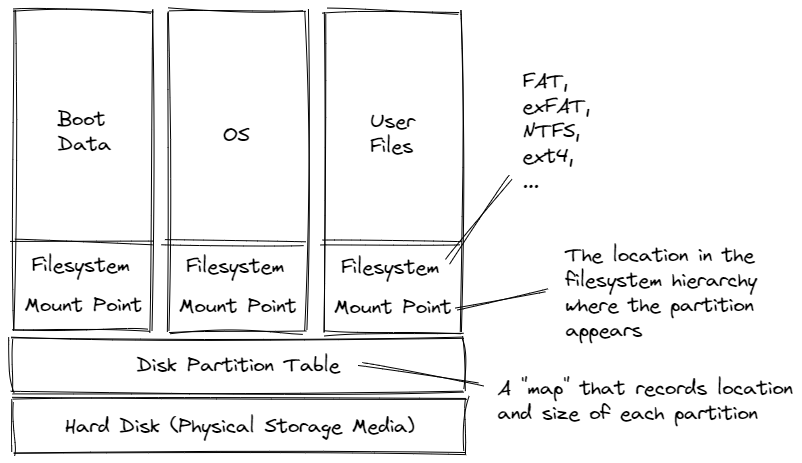
\includegraphics[width=300pt]{chapters/part-2/figures/partition.png}
	\caption{A demonstration of how a hard drive is used in the OS.} \label{ch:dm:fig:partition}
\end{figure}

Usually, each filesystem is associated with a partition. The partition focuses more on the logical separation of the hard drive, while the filesystem focuses more on how the operating system manages the data within that partition. Ideally they are consistent and there should be a clear correspondence. However, it is possible that when the filesystem is not sized correctly, the filesystem is smaller than its associated partition, and a part of the storage becomes unused. A filesystem is only meaningful on a partition because it describes how that partition is formatted and managed. Therefore, a filesystem cannot exist without a partition. However, a partition can exist without a filesystem. It will be an unused storage space that is not useful to the operating system until it is formatted with a filesystem.

A demonstration of partitions versus filesystems is given in Fig. \ref{ch:dm:fig:partitionvsfilesystem}.

\begin{figure}[htbp]
	\centering
	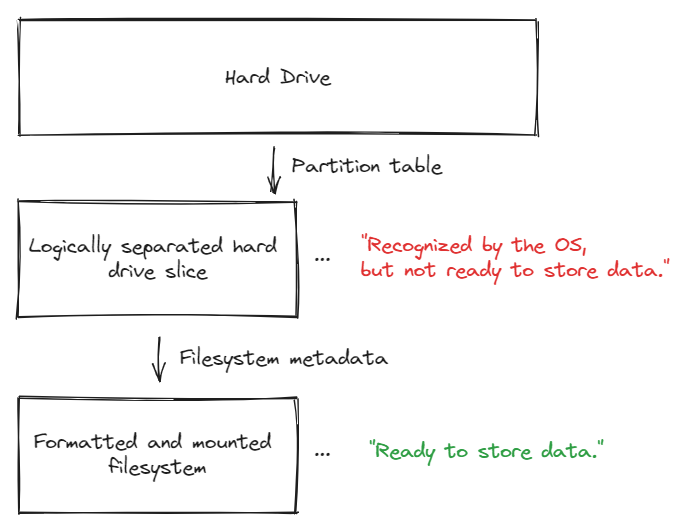
\includegraphics[width=300pt]{chapters/part-2/figures/partitionvsfilesystem.png}
	\caption{A demonstration of how partitions and filesystems relate to each other.} \label{ch:dm:fig:partitionvsfilesystem}
\end{figure}


Use \verb|df| to monitor the status of the mounted storage, including the filesystem name, size, and used percentage. Command \verb|df -h| gives a nice snapshot of the storage usage in a human-readable format. An example is given below.
\begin{lstlisting}
$ df -h
Filesystem      Size  Used Avail Use% Mounted on
tmpfs           1.2G  2.1M  1.2G   1% /run
/dev/sda3       916G   51G  818G   6% /
tmpfs           5.8G     0  5.8G   0% /dev/shm
tmpfs           5.0M  4.0K  5.0M   1% /run/lock
/dev/sda2       512M  5.3M  507M   2% /boot/efi
tmpfs           1.2G  120K  1.2G   1% /run/user/1000
\end{lstlisting}
from where it can be seen that the most of the storage of the system, in this case $818G$, is mounted on the root directory.

Use \verb|lsblk| to list information about block devices in the OS. Block devices refer to nonvolatile mass storage devices whose information can be accessed in any order, such as hard disks and CD-ROMs. An example is given below.
\begin{lstlisting}
$ lsblk
NAME   MAJ:MIN RM   SIZE RO TYPE MOUNTPOINTS
loop0    7:0    0     4K  1 loop /snap/bare/5
loop1    7:1    0    62M  1 loop /snap/core20/1593
loop2    7:2    0    62M  1 loop /snap/core20/1611
loop3    7:3    0 163.3M  1 loop /snap/firefox/1670
loop4    7:4    0   177M  1 loop /snap/firefox/1749
loop5    7:5    0 400.8M  1 loop /snap/gnome-3-38-2004/112
loop6    7:6    0 248.8M  1 loop /snap/gnome-3-38-2004/99
loop7    7:7    0  81.3M  1 loop /snap/gtk-common-themes/1534
loop8    7:8    0  91.7M  1 loop /snap/gtk-common-themes/1535
loop9    7:9    0  45.9M  1 loop /snap/snap-store/575
loop10   7:10   0    47M  1 loop /snap/snapd/16010
loop11   7:11   0  45.9M  1 loop /snap/snap-store/582
loop12   7:12   0    47M  1 loop /snap/snapd/16292
loop13   7:13   0   284K  1 loop /snap/snapd-desktop-integration/10
loop14   7:14   0   284K  1 loop /snap/snapd-desktop-integration/14
sda      8:0    0 931.5G  0 disk
|-sda1   8:1    0     1M  0 part
|-sda2   8:2    0   513M  0 part /boot/efi
|-sda3   8:3    0   931G  0 part /
sr0     11:0    1  1024M  0 rom
\end{lstlisting}
which gives the size, the type and the mount point of all the storages.

Use \verb|blkid| to print block device attributes. An example is given below.
\begin{lstlisting}
$ blkid
/dev/sda3: UUID="d0b15b7c-71f2-41f4-b67a-e7c69446feab" BLOCK_SIZE="4096" TYPE="ext4" PARTUUID="4b570507-6aa0-46c7-ac1b-06cb4c8bdb61"
\end{lstlisting}

\section{Disk Partition Table Manipulation}

Due to the development of computer science and OS, manual disk partition is less necessary than before for a casual user. Nevertheless, Linux provides necessary tools for disk partition table manipulation and they are introduced in this section.

\subsection{Disk Partition}

Disk partitioning refers to the action of creating one or more regions on secondary storage (e.g., disk) so that they can be managed separately, as if they are different ``virtual disks''. An example of disk partitioning on a Windows PC would be to partition a $1TB$ hard drive into $512GB$ of \verb|C:\| drive and $512GB$ of \verb|D:\| drive. Partitioned regions are logically separated. The partitions locations and sizes are stored in the disk partition table.

Some of the reasons for using disk partition include:
\begin{itemize}
  \item Due to capability limitation, OS cannot handle a very large disk storage as a whole (this is less the case nowadays).
  \item Different types of files, for example system data and user data, can be stored separately for easy management.
  \item Different filesystems can be used on different partitions.
  \item Different partitions can be configured differently with unique settings.
  \item Sometimes partitioning can speed up hard disk accessing.
\end{itemize}

\subsection{Disk Partition Table Manipulation}

From the output of \verb|lsblk| command earlier, it is clear that the system's hard disk name is ``\verb|sda|''. To get a bit more details on this disk and its current partitioning status, use
\begin{lstlisting}
$ sudo fdisk -l | grep sda
Disk /dev/sda: 931.51 GiB, 1000204886016 bytes, 1953525168 sectors
/dev/sda1     2048       4095       2048    1M BIOS boot
/dev/sda2     4096    1054719    1050624  513M EFI System
/dev/sda3  1054720 1953523711 1952468992  931G Linux filesystem
\end{lstlisting}

From the above result, it can be seen that the disk registered under \verb|/dev/| (this is where the devices are represented by default) has been partitioned into 3 partitions, and the user space that can be further modified is \verb|/dev/sda3| which is $931GB$.

There are variety of tools that can be used for disk partitioning. A common way of doing that is to use
\begin{lstlisting}
$ sudo fdisk /dev/sda3
\end{lstlisting}
to enter the fdisk utility, and follow the wizard.

Other tools such as \verb|cfdisk| and \verb|parted| can also be used similarly for disk partition.

\section{Mount, Unmount and Format a Partition}

The hard disk can be formatted by partition, from where a new filesystem can be created. To format a partition, double check using \verb|lsblk| to make sure that it is not mounted in the system. Use \verb|sudo umount <partition name>| to unmount a partition.

Use \verb|sudo mkfs| to format and create a new formatted filesystem, then use \verb|mount| to mount it back to the OS. The mount of a partition needs to be recorded into \verb|/etc/fstab| so that the OS would remember it after a reboot.
